% Options for packages loaded elsewhere
\PassOptionsToPackage{unicode}{hyperref}
\PassOptionsToPackage{hyphens}{url}
%
\documentclass[
]{article}
\usepackage{lmodern}
\usepackage{amssymb,amsmath}
\usepackage{ifxetex,ifluatex}
\ifnum 0\ifxetex 1\fi\ifluatex 1\fi=0 % if pdftex
  \usepackage[T1]{fontenc}
  \usepackage[utf8]{inputenc}
  \usepackage{textcomp} % provide euro and other symbols
\else % if luatex or xetex
  \usepackage{unicode-math}
  \defaultfontfeatures{Scale=MatchLowercase}
  \defaultfontfeatures[\rmfamily]{Ligatures=TeX,Scale=1}
\fi
% Use upquote if available, for straight quotes in verbatim environments
\IfFileExists{upquote.sty}{\usepackage{upquote}}{}
\IfFileExists{microtype.sty}{% use microtype if available
  \usepackage[]{microtype}
  \UseMicrotypeSet[protrusion]{basicmath} % disable protrusion for tt fonts
}{}
\makeatletter
\@ifundefined{KOMAClassName}{% if non-KOMA class
  \IfFileExists{parskip.sty}{%
    \usepackage{parskip}
  }{% else
    \setlength{\parindent}{0pt}
    \setlength{\parskip}{6pt plus 2pt minus 1pt}}
}{% if KOMA class
  \KOMAoptions{parskip=half}}
\makeatother
\usepackage{xcolor}
\IfFileExists{xurl.sty}{\usepackage{xurl}}{} % add URL line breaks if available
\IfFileExists{bookmark.sty}{\usepackage{bookmark}}{\usepackage{hyperref}}
\hypersetup{
  pdftitle={linear norm plot},
  pdfauthor={Joshua},
  hidelinks,
  pdfcreator={LaTeX via pandoc}}
\urlstyle{same} % disable monospaced font for URLs
\usepackage[margin=1in]{geometry}
\usepackage{graphicx,grffile}
\makeatletter
\def\maxwidth{\ifdim\Gin@nat@width>\linewidth\linewidth\else\Gin@nat@width\fi}
\def\maxheight{\ifdim\Gin@nat@height>\textheight\textheight\else\Gin@nat@height\fi}
\makeatother
% Scale images if necessary, so that they will not overflow the page
% margins by default, and it is still possible to overwrite the defaults
% using explicit options in \includegraphics[width, height, ...]{}
\setkeys{Gin}{width=\maxwidth,height=\maxheight,keepaspectratio}
% Set default figure placement to htbp
\makeatletter
\def\fps@figure{htbp}
\makeatother
\setlength{\emergencystretch}{3em} % prevent overfull lines
\providecommand{\tightlist}{%
  \setlength{\itemsep}{0pt}\setlength{\parskip}{0pt}}
\setcounter{secnumdepth}{-\maxdimen} % remove section numbering
\usepackage{booktabs}
\usepackage{longtable}
\usepackage{array}
\usepackage{multirow}
\usepackage{wrapfig}
\usepackage{float}
\usepackage{colortbl}
\usepackage{pdflscape}
\usepackage{tabu}
\usepackage{threeparttable}
\usepackage{threeparttablex}
\usepackage[normalem]{ulem}
\usepackage{makecell}
\usepackage{xcolor}

\title{linear norm plot}
\author{Joshua}
\date{15/05/2020}

\begin{document}
\maketitle

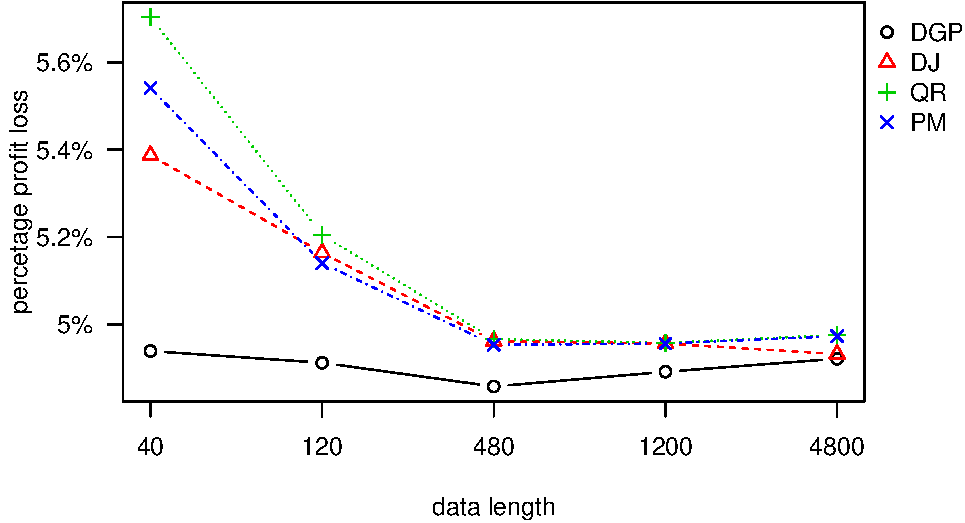
\includegraphics{linear-norm-plot_files/figure-latex/ppl0.5-1.pdf}

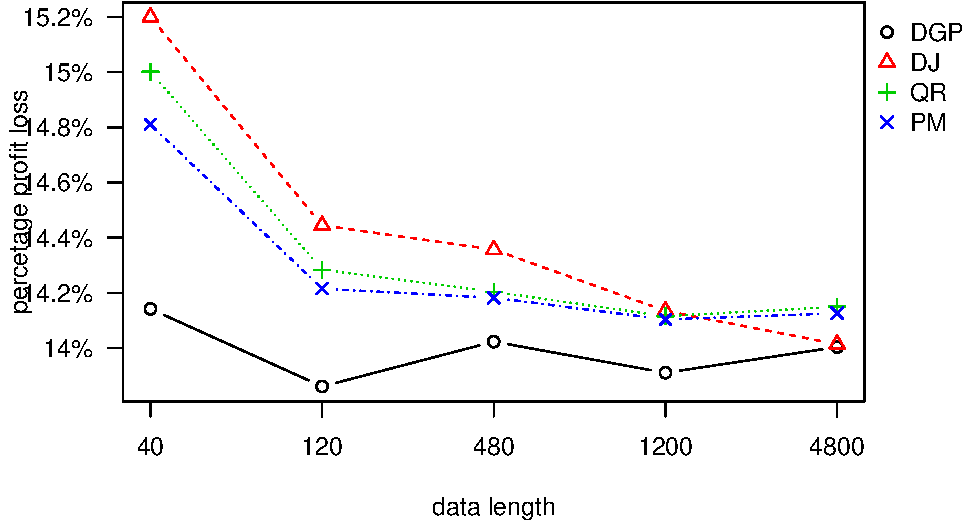
\includegraphics{linear-norm-plot_files/figure-latex/ppl0.63-1.pdf}

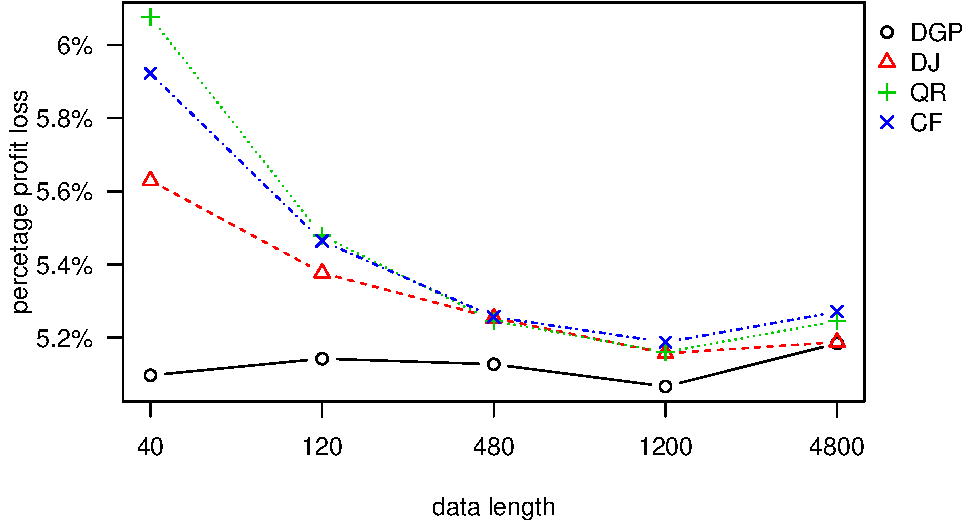
\includegraphics{linear-norm-plot_files/figure-latex/ppl0.3-1.pdf}

\begin{table}

\caption{\label{tab:inventory_error}Inventory Error}
\centering
\resizebox{\linewidth}{!}{
\begin{tabular}[t]{ccccccccccccc}
\toprule
\multicolumn{1}{c}{\textbf{ }} & \multicolumn{4}{c}{\textbf{Target service level=0.5}} & \multicolumn{4}{c}{\textbf{Target service level=0.63}} & \multicolumn{4}{c}{\textbf{Target service level=0.3}} \\
\cmidrule(l{3pt}r{3pt}){2-5} \cmidrule(l{3pt}r{3pt}){6-9} \cmidrule(l{3pt}r{3pt}){10-13}
Data size & DGP & disjoint & quantile & proposed & DGP & disjoint & quantile & proposed & DGP & disjoint & quantile & proposed\\
\midrule
\rowcolor{gray!6}  40 & 0.44 & 31.16 & -0.18 & -0.68 & -68.28 & -45.21 & -67.5 & -64.58 & 104.03 & 148.12 & 102.88 & 101.25\\
 & (199.19) & (221.06) & (216.35) & (214.19) & (199.59) & (221.45) & (216.89) & (214.34) & (200.43) & (223.53) & (219.48) & (217.4)\\
\rowcolor{gray!6}  120 & -0.14 & 12.08 & 0.09 & 0.27 & -68.68 & -61.41 & -68.57 & -67.2 & 106.91 & 127.12 & 107.76 & 106.27\\
 & (197.84) & (209.63) & (204.33) & (203.65) & (200.48) & (212.36) & (206.85) & (206.58) & (199.8) & (211.43) & (206.79) & (206.81)\\
\rowcolor{gray!6}  480 & 0.92 & 4.71 & 0.81 & 0.82 & -70.91 & -70.01 & -71.49 & -70.32 & 105.25 & 111.97 & 106.18 & 104.64\\
\addlinespace
 & (199.61) & (204.63) & (203.02) & (202.8) & (199.46) & (205.28) & (203.23) & (203.2) & (200.2) & (206.2) & (203.63) & (204)\\
\rowcolor{gray!6}  1200 & 0.43 & 2 & 0.37 & 0.38 & -67.39 & -67.33 & -68.14 & -67.16 & 104.48 & 108.36 & 105.78 & 104.37\\
 & (199.83) & (203.83) & (202.4) & (202.36) & (199.93) & (203.55) & (202.63) & (202.8) & (202.2) & (206.16) & (205.02) & (205.47)\\
\rowcolor{gray!6}  4800 & -2.43 & -1.98 & -2.44 & -2.44 & -66.32 & -66.1 & -66.8 & -65.73 & 105.33 & 106.16 & 106.73 & 105.2\\
 & (200.22) & (200.78) & (203.12) & (203.11) & (199.31) & (199.76) & (201.63) & (201.82) & (199.6) & (200.15) & (202.28) & (202.65)\\
\bottomrule
\end{tabular}}
\end{table}

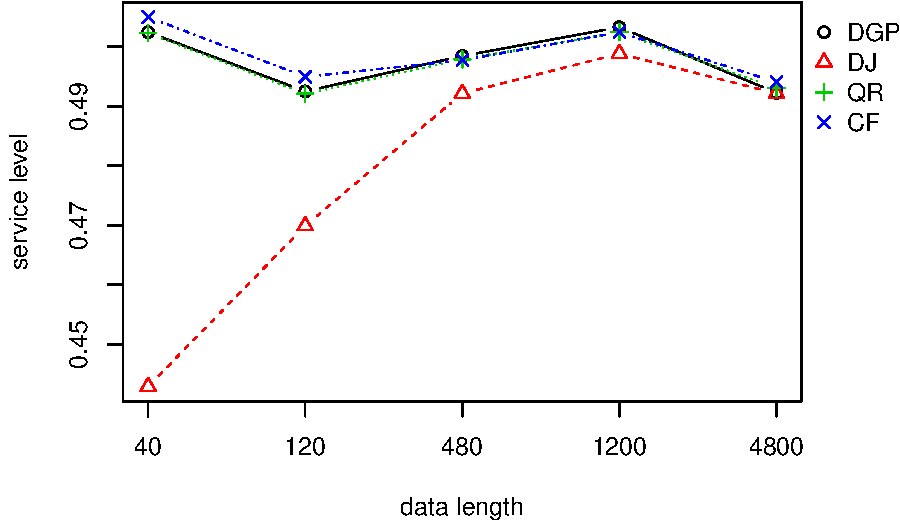
\includegraphics{linear-norm-plot_files/figure-latex/sl-1.pdf}
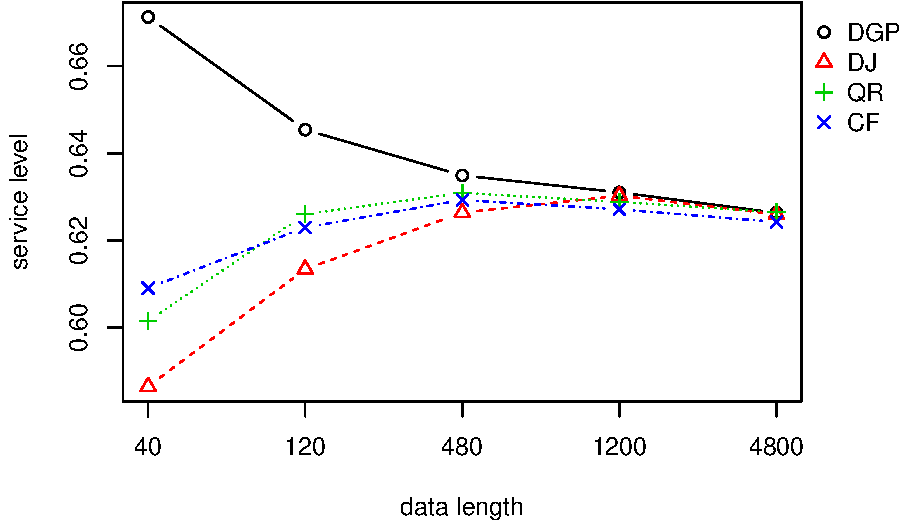
\includegraphics{linear-norm-plot_files/figure-latex/sl-2.pdf}
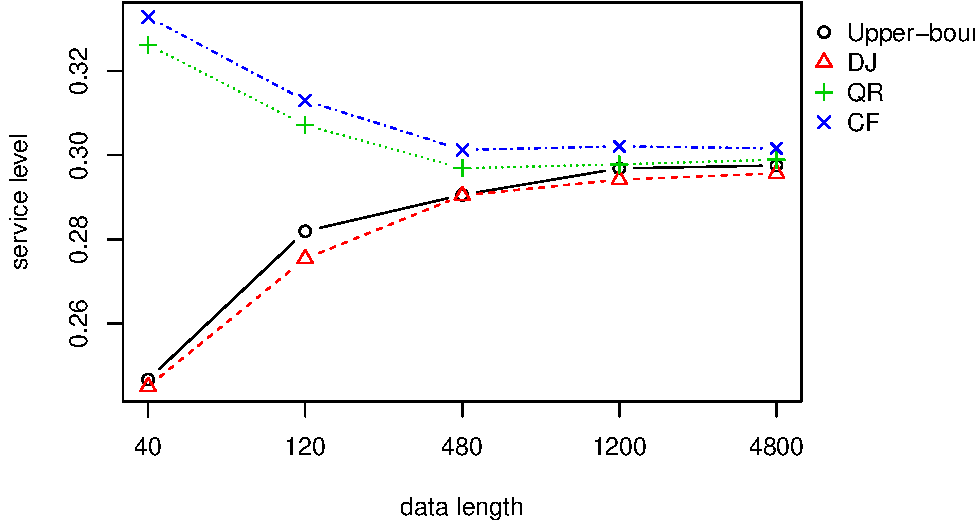
\includegraphics{linear-norm-plot_files/figure-latex/sl-3.pdf}
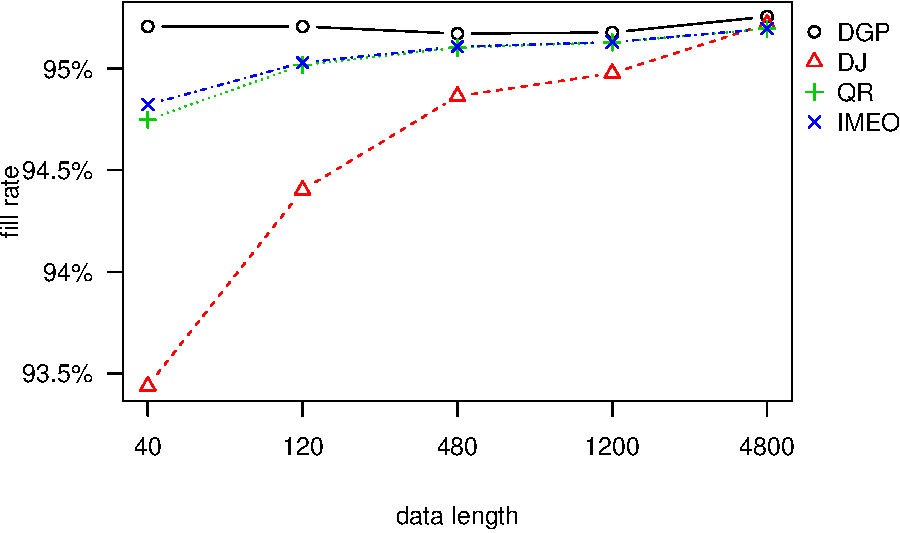
\includegraphics{linear-norm-plot_files/figure-latex/fr-1.pdf}
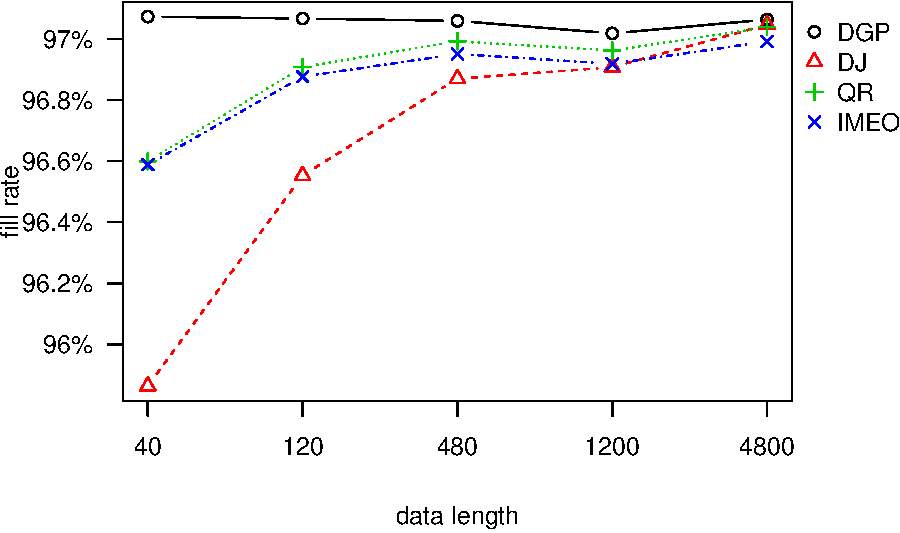
\includegraphics{linear-norm-plot_files/figure-latex/fr-2.pdf}
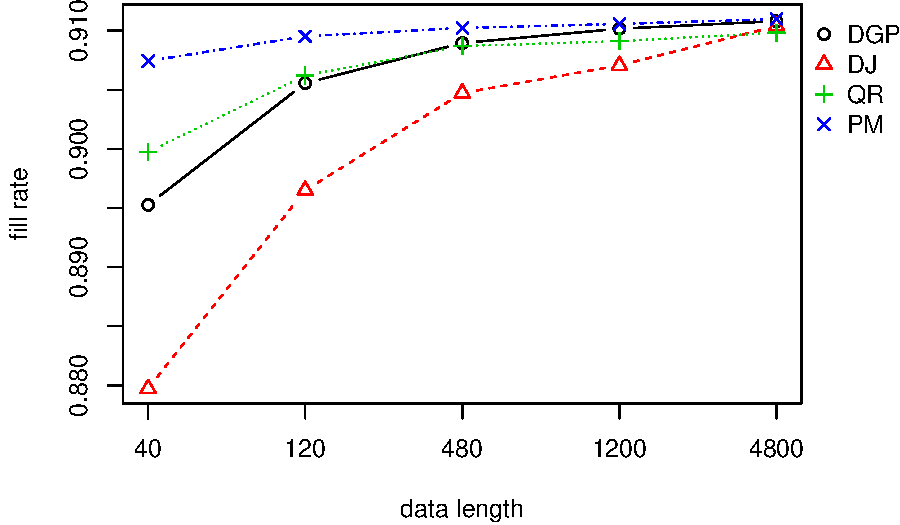
\includegraphics{linear-norm-plot_files/figure-latex/fr-3.pdf}

\begin{table}

\caption{\label{tab:Wilcoxon}p-value of Wilcoxon Test between data size 1200 and 4800}
\centering
\begin{tabular}[t]{ccccc}
\toprule
Target service level & DGP & disjoint & quantile & proposed\\
\midrule
\rowcolor{gray!6}  0.5 & 0.8180896 & 0.5092581 & 0.7871617 & 0.6599393\\
0.63 & 0.4012898 & 0.6338719 & 0.1681950 & 0.1528860\\
\rowcolor{gray!6}  0.3 & 0.7193090 & 0.5123136 & 0.8959545 & 0.8109658\\
\bottomrule
\end{tabular}
\end{table}

\begin{table}[H]
\centering
\resizebox{\linewidth}{!}{
\begin{tabular}{ccccccccccccc}
\toprule
\multicolumn{1}{c}{\textbf{ }} & \multicolumn{4}{c}{\textbf{Percentage profit loss}} & \multicolumn{4}{c}{\textbf{Service level}} & \multicolumn{4}{c}{\textbf{Fill rate}} \\
\cmidrule(l{3pt}r{3pt}){2-5} \cmidrule(l{3pt}r{3pt}){6-9} \cmidrule(l{3pt}r{3pt}){10-13}
Data size & DGP & DJ & QR & IMEO & DGP & DJ & QR & IMEO & DGP & DJ & QR & IMEO\\
\midrule
40 & 5.2\% & 5.6\% & 5.7\% & 5.6\% & 0.3 & 0.26 & 0.32 & 0.32 & 91.1\% & 88.2\% & 90.6\% & 90.8\%\\
120 & 5.1\% & 5.4\% & 5.3\% & 5.3\% & 0.3 & 0.27 & 0.30 & 0.30 & 91.0\% & 89.6\% & 90.8\% & 90.9\%\\
480 & 5.2\% & 5.3\% & 5.2\% & 5.3\% & 0.3 & 0.29 & 0.30 & 0.30 & 91.0\% & 90.5\% & 90.9\% & 91.0\%\\
1200 & 5.2\% & 5.3\% & 5.3\% & 5.4\% & 0.3 & 0.30 & 0.30 & 0.30 & 91.0\% & 90.7\% & 90.9\% & 91.0\%\\
4800 & 5.1\% & 5.1\% & 5.2\% & 5.2\% & 0.3 & 0.30 & 0.30 & 0.30 & 91.1\% & 91.0\% & 91.0\% & 91.1\%\\
\bottomrule
\end{tabular}}
\end{table}

\begin{table}[H]
\centering
\resizebox{\linewidth}{!}{
\begin{tabular}{ccccccccccccc}
\toprule
\multicolumn{1}{c}{\textbf{ }} & \multicolumn{4}{c}{\textbf{Percentage profit loss}} & \multicolumn{4}{c}{\textbf{Service level}} & \multicolumn{4}{c}{\textbf{Fill rate}} \\
\cmidrule(l{3pt}r{3pt}){2-5} \cmidrule(l{3pt}r{3pt}){6-9} \cmidrule(l{3pt}r{3pt}){10-13}
Target service level & DGP & DJ & QR & IMEO & DGP & DJ & QR & IMEO & DGP & DJ & QR & IMEO\\
\midrule
0.5 & 4.9\% & 5.3\% & 5.3\% & 5.2\% & 0.50 & 0.44 & 0.50 & 0.50 & 95.2\% & 93.4\% & 94.7\% & 94.8\%\\
0.63 & 13.8\% & 15.1\% & 15.0\% & 14.8\% & 0.63 & 0.58 & 0.62 & 0.62 & 97.1\% & 95.8\% & 96.6\% & 96.6\%\\
0.3 & 5.2\% & 5.6\% & 5.7\% & 5.6\% & 0.30 & 0.26 & 0.32 & 0.32 & 91.1\% & 88.2\% & 90.6\% & 90.8\%\\
\bottomrule
\end{tabular}}
\end{table}

\begin{table}[H]
\centering
\resizebox{\linewidth}{!}{
\begin{tabular}{ccccccccccccc}
\toprule
\multicolumn{1}{c}{\textbf{ }} & \multicolumn{4}{c}{\textbf{Percentage profit loss}} & \multicolumn{4}{c}{\textbf{Service level}} & \multicolumn{4}{c}{\textbf{Fill rate}} \\
\cmidrule(l{3pt}r{3pt}){2-5} \cmidrule(l{3pt}r{3pt}){6-9} \cmidrule(l{3pt}r{3pt}){10-13}
Target service level & DGP & DJ & QR & IMEO & DGP & DJ & QR & IMEO & DGP & DJ & QR & IMEO\\
\midrule
0.5 & 4.9\% & 4.9\% & 5.0\% & 5.0\% & 0.50 & 0.50 & 0.50 & 0.50 & 95.3\% & 95.2\% & 95.2\% & 95.2\%\\
0.63 & 13.8\% & 13.8\% & 14.0\% & 14.0\% & 0.63 & 0.63 & 0.63 & 0.63 & 97.0\% & 97.0\% & 97.0\% & 96.9\%\\
0.3 & 5.1\% & 5.1\% & 5.2\% & 5.2\% & 0.30 & 0.30 & 0.30 & 0.30 & 91.1\% & 91.0\% & 91.0\% & 91.1\%\\
\bottomrule
\end{tabular}}
\end{table}

\end{document}
